\documentclass[a4paper,11pt]{report}

\usepackage[frenchb]{babel}
\usepackage[utf8]{inputenc}
\usepackage{wrapfig}
\usepackage{graphicx}
\usepackage {amsmath}
\usepackage{amssymb}
\usepackage{amsthm}
\usepackage{mathrsfs}
\usepackage{soul}
\usepackage{algorithm,algorithmic}
\usepackage{listings}
\usepackage{array}
\usepackage[top=2.5cm, bottom=3cm, left=3cm, right=3cm]{geometry}


\begin{document}

%%%%%%%%%%%%%%%%%%%%%%%%%%%%%%%%%%%%%%%%%%%%%%%%%%%
%page de garde
\begin{figure}
   
\includegraphics[scale = 0.75]{HeaderPagedeGarde.PNG}
\end{figure}


\author{Maxime Escourbiac - Jean-Christophe Septier \\ Responsable ISIMA : David HILL}
\title{
   Rapport de travaux pratiques \\ 3ème année ingénieur \\ Génie logiciel et Systèmes Informatiques \\
  \bigskip
   \large{
      Ingénierie des modèles \& Simulation
   }
}
\date{9 Novembre 2011}
\maketitle

\newpage

%%%%%%%%%%%%%%%%%%%%%%%%%%%%%%%%%%%%%%%%%%%%%%%%%%%

\begin{flushleft}
\LARGE{ \underline {Résumé :}\bigskip}
\end{flushleft}

\normalsize{
Ces travaux sont dans dans la continuité du rapport précédent. Ils ont permis d'approfondir le concept de "métaprogrammation" en l'appliquant au domaine de la simulation. La première partie de l'étude, présente, dans ce rapport montre un benchmark des performances d'une simulation de Monte-Carlo ( calcul de PI ) des différentes méthodes de programmation afin d'en quantifier leurs forces et leurs faiblesses. La seconde propose un méta-modèle du langage C++ qui a pour but final la génération de "Header" en langage C++ puis si possible en langage Java.
}

\begin{flushleft}
\large{ \underline {Mots-clés:}\bigskip}\\
{\bf   Métaprogrammation, Ingénierie des modèles, Simulation, C++ ,Java}
\end{flushleft}

\newpage

%%%%%%%%%%%%%%%%%%%%%%%%%%%%%%%%%%%%%%%%%%%%%%%%%%%

%%%%%%%%%%%%%%%%%%%%%%%%%%%%%%%%%%%%%%%%%%%%%%%%%%%%
%table des matieres

\tableofcontents
\newpage

\listoffigures
\newpage

%%%%%%%%%%%%%%%%%%%%%%%%%%%%%%%%%%%%%%%%%%%%%%%%%%%

\begin{flushleft}
\LARGE{ \underline {Introduction :}\bigskip}
\end{flushleft}

\normalsize{
Le cours de simulation de deuxième année nous as apporté des méthodes pour correctement modélisé un problème afin de le simuler. Cette partie du cours d'ingénierie des modèles traite en parti des optimisations du code afin de les rendre plus efficaces. L'une de ces méthodes consiste à utilisé la métaprogrammation pour améliorer le temps de génération de nombre aléatoire. Nous verrons dans ce compte-rendu comment l'implémenter et observer l'impact sur les performances de la simulation. \\
}

\normalsize{
Le langage C++ est considéré comme un des langages des plus complet. En effet, on peut mettre en place de très nombreux concepts de programmation ( l'objet, la programmation par aspect avec AspectC++, la métaprogrammation, la programmation récursive etc... ) grâce aux différents mécanismes du langage. Pour mieux le comprendre et se l'approprier, on a construit un métamodèle simplifié du C++ qui mettra en évidence les liaisons entre les différents éléments du langage. Cette construction permettra à terme de générer du code source en C++ puis en langage Java. Ce point touche une des faiblesses qui est l'absence d'instrospection et de reflexion, domaines observés lors du premier TP.
}

%%%%%%%%%%%%%%%%%%%%%%%%%%%%%%%%%%%%%%%%%%%%%%%%%%%%%%%%%%%%%%%%%%%%%

\chapter {La métaprogrammation dans la simulation}

\section{ Mersenne Twister}

\normalsize{
Initié par {\bf Makoto Matsumoto} en 1997, le Mersenne Twister est un générateur de nombres pseudo-aléatoires réputé pour sa qualité. Son implémentation est inséré dans le standard de la norme C++11. L'algorithme est basé sur un TGSFR (twisted generalised shift feedback register, un type particulier de registre à décalage à rétroaction) et tient son nom d'un nombre premier de Mersenne. Il existe au moins deux variantes majeures, la plus répandue étant MT 19937, utilisant le nombre premier de Mersenne  et présente les propriétés suivantes : \\
}

\begin{itemize}
    \item Sa période est de $ 2^{19937} - 1 $ .
    \item Il est uniformément distribué sur un grand nombre de dimensions (623 pour les nombres de 32 bits).
    \item Il est plus rapide que la plupart des autres générateurs (sauf les plus médiocres statistiquement) .
    \item Il est aléatoire quel que soit le poids du bit considéré, et passe les tests Diehard$^1$ \footnotetext[1]{Les diehard tests sont une batterie de tests statistiques pour mesurer la qualité d'un générateur. } \\
\end{itemize}

\normalsize{
L'initialisation de ce générateur peut se faire de deux façon, soit en utilisant un nombre, soit en utilisant un tableau. Il est conseillé de l'initialiser de la forme suivante : 
}

\begin{lstlisting}[language=C++]
int i;
unsigned long init[4]={0x123, 0x234, 0x345, 0x456}, length=4;
init_by_array(init, length);
\end{lstlisting}

\normalsize{
Ces valeurs d'initialisation seront conservées pour toute la suite du TP, afin de pouvoir obtenir des résultats comparables.
}


\section{La génération de code}

\normalsize{
L'une des optimisation proposée sur ce tp est la génération automatique du code source  de la simulation.En effet, le temps d'appel au générateur n'est plus négligeable pour un très grand nombre tiré. Le but est donc, de généré un code source où les nombres aléatoires seront directement intégrées dans un tableau en variable globale donc ainsi la simulation ne fera en aucun cas d'appel au générateur. Celui-ci étant utilisé seulement par le métaprogramme. Voici un schéma montrant le principe de l'amélioration.
}

\clearpage

\begin{figure}[h]
   \begin{center}
   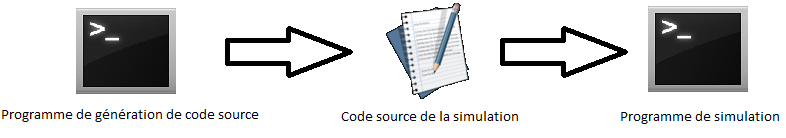
\includegraphics[scale = 0.7]{generationdecode.PNG}
   \end{center}
  \caption{Principe de la métaprogrammation}
\end{figure}

\normalsize{
\noindent
Voici un exemple d'un code source généré par métaprogrammation qu'on peut obtenir en sortie.
}

\begin{lstlisting}[language=C++]

#include xxxxx

float mt[] = {
0.2345535,
0.7647367,
...
}

int main(int argc, char ** argv)
{
//Traitement
}
\end{lstlisting}

\vspace{0.5cm}
\normalsize{
\noindent
Les résultats intéressant à observer sont: \\
}

\begin{itemize}
    \item Le temps de génération du code source de la simulation.
    \item Le temps de compilation du code source de la simulation.
    \item Le temps d'exécution de la simulation. \\
\end{itemize}

\normalsize{
Les méthodes de mesures et les résultats seront analysés dans la section benchmark du rapport. \\
} 


\section {Memory Mapping}

\subsection{La théorie}
  
\normalsize{
Il est parfois intéressant, plutôt que de travailler sur le contenu d'un fichier, d'en projeter une image en mémoire, sur laquelle on œuvre ensuite comme avec des variables normales. Cette projection permet de manipuler le contenu du fichier au moyen d'une image en mémoire, donc beaucoup plus rapidement et simplement qu'avec des véritables lectures et écritures sur le disque. Sur UNIX/Linux cette opération se fait avec l'appel système mmap() déclaré dans $<$sys/mman.h$>$ et donc voici le prototype.
}

\begin{lstlisting}[language=C++]
void * mmap ( void * debut, size_t longueur, int protection,
              int attribut, int fd, off_t offset);
\end{lstlisting}


\subsection{La pratique dans le domaine de simulation}

\normalsize{
Le principe de memory mappinng en simulation reprend le concept d'externalisation de la génération de nombre aléatoire. En effet la séquence de nombres aléatoire est générée par un programme annexe. A la différence du métaprogramme précédent, les tirages sont stockés dans un fichier. La simulation pourra donc se servir de ces fichiers pour "simuler" un générateur. La solution retenu pour exploiter cette ressource a été le memory mapping qui a été décrit dans la sous-section ci-dessus. Voici un schéma reprenant l'idée du memory mapping pour une simulation.
}

\begin{figure}[h]
   \begin{center}
   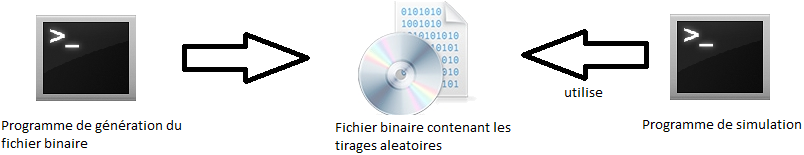
\includegraphics[scale = 0.65]{generationmmap.PNG}
   \end{center}
  \caption{Memory mapping utilisé en simulation}
\end{figure}



\section{Benchmark}

\subsection{Procedures de test}

\normalsize{
Le contexte de test est le calcul de l'approximation de PI ( code réalisé en deuxième année lors du cours de simulation ).  Les paramètres de test seront les nombres de réplications et le nombres de point (x,y) utilises. Voici l'algorithme utilise pour approximer pi. \\
}

\begin{algorithm}[h]
\caption{Approximation de PI}
\begin{algorithmic}
\STATE $valide = 0$
\FOR{$i = 1 \to NBTIRAGE$} 
\STATE $ x \gets rand()$
\STATE $ y \gets rand()$
\IF{ $x^2 + y^2 < 1$}
 \STATE valide++
\ENDIF
\ENDFOR
\RETURN $ (4 . valide) / NBTIRAGE $
\end{algorithmic}
\end{algorithm}

\normalsize{
Tous les codes sources utilises pour le benchmark ont été compilé à l'aide de GCC ou G++ avec l'option -O2. Les exécutions ont été faite sur un serveur personnel bi-processeur tournant sur Debian 6.0. 
} 

\subsection{Test de performance sur la génération de code}

\normalsize{
La première partie du test est sur le temps de génération du code source. Le code a été développé en C++. Le fichier obtenu en sortie correspond au code source de la simulation prêt à être compile.Les résultats ont été obtenues suite à la moyenne de 10 mesures de temps de génération de code. Voici les graphe représentant les temps d'exécution pour ce programme pour 5 réplications puis 10 réplications.
}

\clearpage

\begin{figure}[h]
\begin{center}
\begin{tabular}{|c|c|c|c|c|c|}
\hline
Nombre de points tirés & 1000 & 10000 & 100000 & 500000 & 1000000 \\
\hline
Temps de génération du code (s) & 0,1035 & 1,0492 & 10,271 & 50,038 & 104,46 \\
\hline
\end{tabular}
\end{center}
\caption{Tableau des résultats pour la génération de code source pour 5 réplications.}
\end{figure}


\begin{figure}[h]
   \begin{center}
   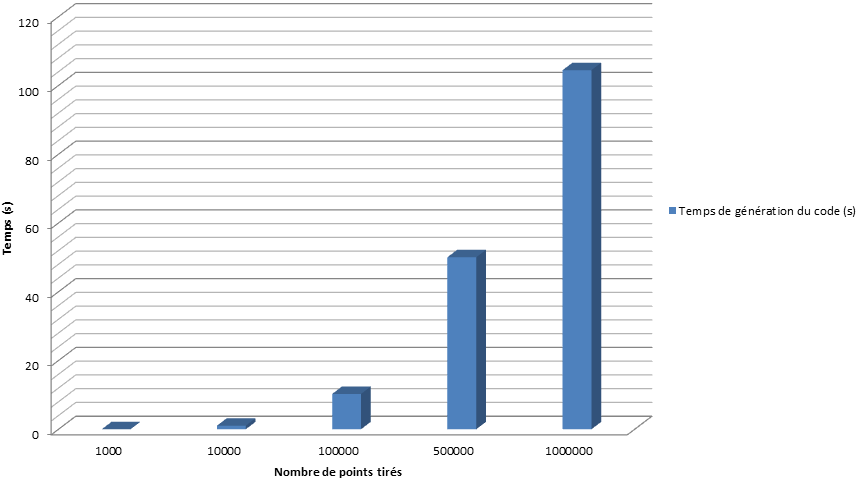
\includegraphics[scale = 0.55]{grapheGenerationCode5.PNG}
   \end{center}
  \caption{Histogramme du temps de génération du code source pour 5 réplications}
\end{figure}

\begin{figure}[h]
\begin{center}
\begin{tabular}{|c|c|c|c|c|c|}
\hline
Nombre de points tirés & 1000 & 10000 & 100000 & 500000 & 1000000 \\
\hline
Temps de génération du code (s) & 0,2077 & 2,0835 & 20,175 & 103,67 & 202,54 \\
\hline
\end{tabular}
\end{center}
\caption{Tableau des résultats pour la génération de code source pour 10 réplications.}
\end{figure}


\begin{figure}[!h]
   \begin{center}
   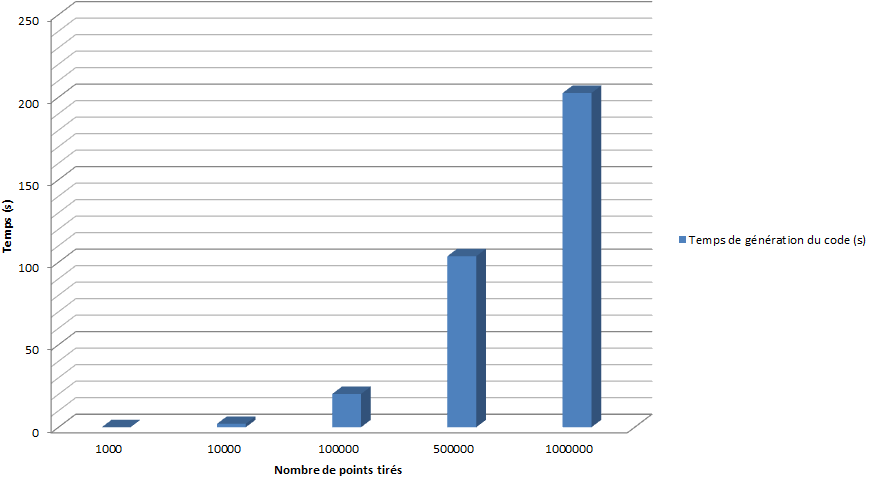
\includegraphics[scale = 0.55]{grapheGenerationCode10.PNG}
   \end{center}
  \caption{Histogramme du temps de génération du code source pour 10 réplications}
\end{figure}

\clearpage

\normalsize{
On remarque que le temps de génération du code est proportionnel au nombre de points tirés. D'un point de vue pratique, dès que le nombre de points est supérieur à 100000. le temps de génération de code commence à ne plus être négligeable pour une simulation.
} 

\subsection{Test de performance de compilation du code source}

\normalsize{
Nous allons voir par la suite les conséquences de l'intégration en variable globale du tableau de nombres aléatoires tirés sur la compilation. En effet, pour une 1000000 de points tirés, le code source obtenu pèse plus de 400mo ce qui est très différent du code de quelques kilo-octets du code original. A titre de comparaison le code classique compile en {\bf 0,264 s} et le code utilisant le memory mapping en {\bf 0,326 s} ( moyenne de 10 compilations  ).Voici les tableaux récapitulatifs et les histogrammes des résultats. \\
}
\begin{figure}[h]
\begin{center}
\begin{tabular}{|c|c|c|c|c|c|}
\hline
Nombre de points tirés & 1000 & 10000 & 100000 & 500000 & 1000000 \\
\hline
Temps de compilation du code (s) & 0,36 & 1,01864 & 16,725 & 91,198 & 215,63 \\
\hline
\end{tabular}
\end{center}
\caption{Tableau des résultats pour la compilation du code source pour 5 réplications.}
\end{figure}

\vspace{0.5cm}

\begin{figure}[!h]
   \begin{center}
   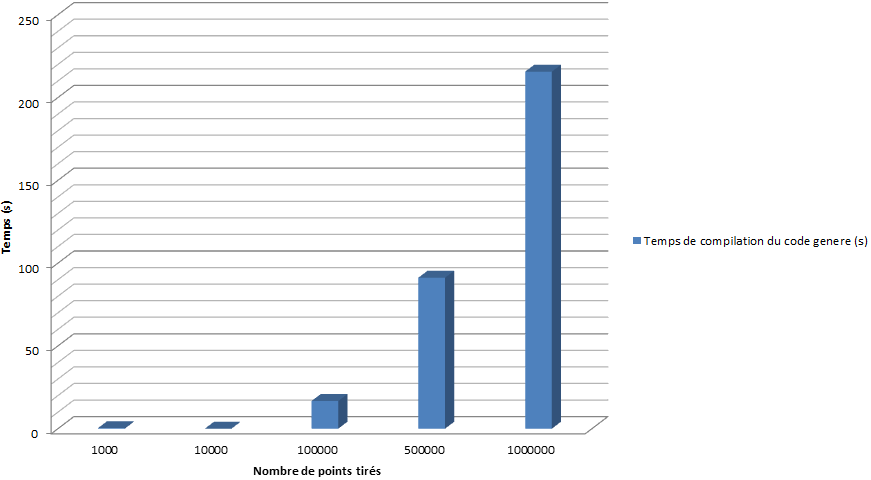
\includegraphics[scale = 0.65]{grapheCompilationCode5.PNG}
   \end{center}
  \caption{Histogramme du temps de compilation du code source pour 5 réplications}
\end{figure}

\vspace{0.5cm}

\begin{figure}[h]
\begin{center}
\begin{tabular}{|c|c|c|c|c|c|}
\hline
Nombre de points tirés & 1000 & 10000 & 100000 & 500000 & 1000000 \\
\hline
Temps de compilation du code (s) & 0,524 & 3,544 & 33,986 & 214,02 & N/A
 \\
\hline
\end{tabular}
\end{center}
\caption{Tableau des résultats pour la compilation du code source pour 10 réplications.}
\end{figure}

 \clearpage
\begin{figure}[!h]
   \begin{center}
   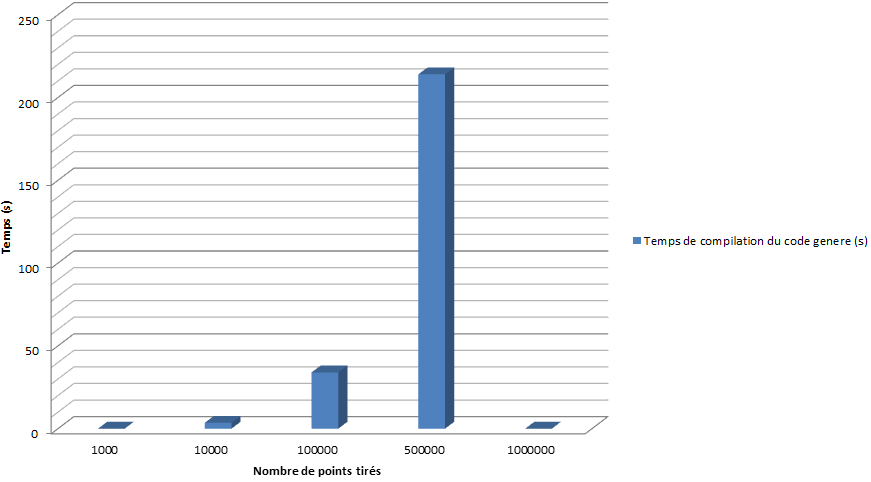
\includegraphics[scale = 0.65]{grapheCompilationCode10.PNG}
   \end{center}
  \caption{Histogramme du temps de compilation du code source pour 10 réplications}
\end{figure}

\normalsize{
Le test pour 1000000 de points tirée pour 10 réplications ne donne pas de résultats à cause de la non-capacité de la machine à compiler ( RAM insuffisante ). On remarque que pour de grand nombre de tirages le temps de compilation augmente. De plus ce type de compilation nécessite une machine ayant une grande mémoire ( $>$ à 10go). Cette étape du processus pourrait être un frein dans le choix du type d'implémentation que l'on souhaiterait.
}

\subsection{Test de performance de la génération du fichier binaire pour le memory mapping}

\normalsize{
Nous allons maintenant tester les temps de génération des fichiers binaires qui seront les ressources utilisées par le programme utilisant le memory mapping. Le fichier obtenu est de forme binaire et est écrit en une seule ligne, à l'aide de la routine {\bf fwrite}. Ce qui permet d'économiser un grand temps d'accès au disque. Voici les tableaux récapitulatifs et les histogrammes des résultats. \\
}

\vspace{0.5cm}

\begin{figure}[h]
\begin{center}
\begin{tabular}{|c|c|c|c|c|c|}
\hline
Nombre de points tirés & 1000 & 10000 & 100000 & 500000 & 1000000 \\
\hline
Temps de génération du fichier (s) & 0,000898 & 0,006889 & 0,066289 & 0,325776 & 0,677531\\
\hline
\end{tabular}
\end{center}
\caption{Tableau des résultats pour la génération du fichier binaire pour 5 réplications.}
\end{figure}

\clearpage

\begin{figure}[!h]
   \begin{center}
   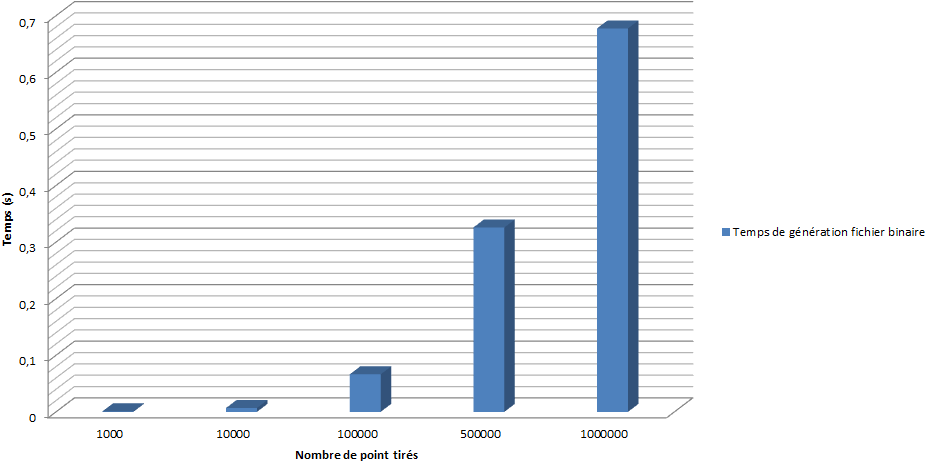
\includegraphics[scale = 0.65]{grapheGenerationfichier5.PNG}
   \end{center}
  \caption{Histogramme du temps de génération du fichier binaire pour 5 réplications}
\end{figure}

\vspace{0.5cm}

\begin{figure}[h]
\begin{center}
\begin{tabular}{|c|c|c|c|c|c|}
\hline
Nombre de points tirés & 1000 & 10000 & 100000 & 500000 & 1000000 \\
\hline
Temps de génération du fichier (s) & 0,001653 & 0,013319 & 0,130788 & 0,767392 & 1,43415\\
\hline
\end{tabular}
\end{center}
\caption{Tableau des résultats pour la génération du fichier binaire pour 10 réplications.}
\end{figure}


\begin{figure}[!h]
   \begin{center}
   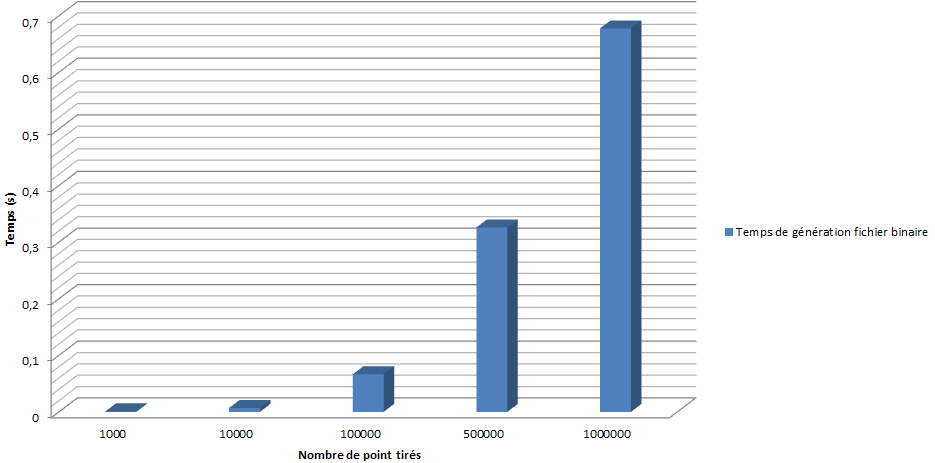
\includegraphics[scale = 0.65]{grapheGenerationfichier10.PNG}
   \end{center}
  \caption{Histogramme du temps de génération du fichier binaire pour 10 réplications}
\end{figure}

\clearpage 

\normalsize{
On remarque que l'écriture de ressources binaires est beaucoup plus efficace que la méthode de métaprogrammation. Si on somme le temps de génération du fichier binaire plus le temps de compilation du code source utilisant le memory mapping, on obtient un résultat très proche du temps du compilation du programme normal. Dans la sous-section suivante, le comparatif des temps d'exécution permettra de savoir si cette méthode est viable.
}

\subsection{Comparatif des temps d'exécution des différentes méthodes}

\normalsize{
Après les mesures des phases préliminaires de chaque méthode, voici le test sur le temps d'exécution de la simulation qui permettra de conclure sur le choix de la méthode la plus efficace parmi les trois.Voici les tableaux récapitulatifs et les histogrammes des résultats.
}

\vspace{0.35cm}

\begin{figure}[h]
\begin{center}
\begin{tabular}{|c|c|c|c|c|c|}
\hline
Nombre de points tirés & 1000 & 10000 & 100000 & 500000 & 1000000 \\
\hline
Classique (s) &0.000736 & 0,006368 & 0,062724 & 0,316108 & 0,675236 \\
\hline
Métaprogrammation (s) & 0.000346 & 0.001706 & 0,015315 & 0,074964 & 0,150158\\
\hline
Memory Mapping (s) & 0,000315 & 0,00217 & 0,019834 & 0,098359 & 0,192794 \\
\hline
\end{tabular}
\end{center}
\caption{Tableau comparatif des temps d'exécution pour 5 répliques.}
\end{figure}

\vspace{0.35cm}

\begin{figure}[!h]
   \begin{center}
   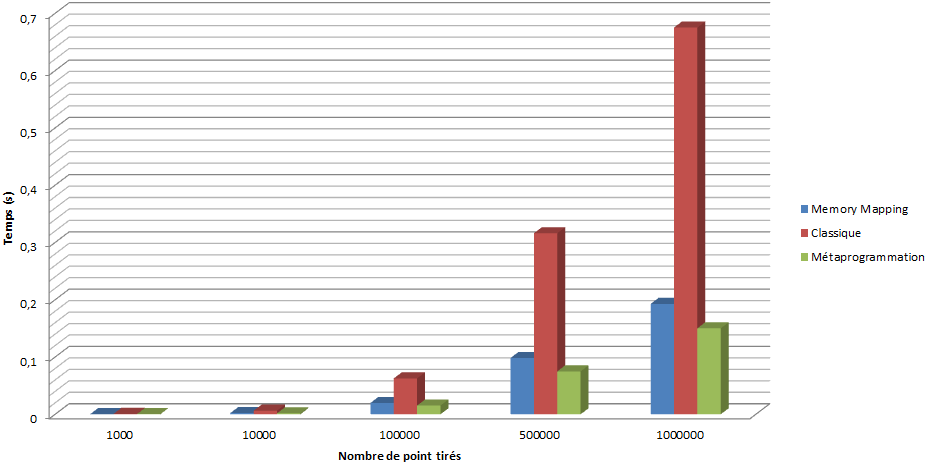
\includegraphics[scale = 0.65]{comparatifResult5.PNG}
   \end{center}
  \caption{Histogramme comparatif des temps d'exécution pour 5 répliques.}
\end{figure}

\begin{figure}[!h]
\begin{center}
\begin{tabular}{|c|c|c|c|c|c|}
\hline
Nombre de points tirés & 1000 & 10000 & 100000 & 500000 & 1000000 \\
\hline
Classique (s) & 0,001434 & 0,012692 & 0,125312 & 0,624241 & 1,250599 \\
\hline
Métaprogrammation (s) & 0,00059 & 0,003552 & 0,032873&  0,170489 & N/A \\
\hline
Memory Mapping (s) & 0,000562 & 0,004125 & 0,039086 & 0,191509 & 0,383219 \\
\hline
\end{tabular}
\end{center}
\caption{Tableau comparatif des temps d'exécution pour 10 répliques.}
\end{figure}

\begin{figure}[!h]
   \begin{center}
   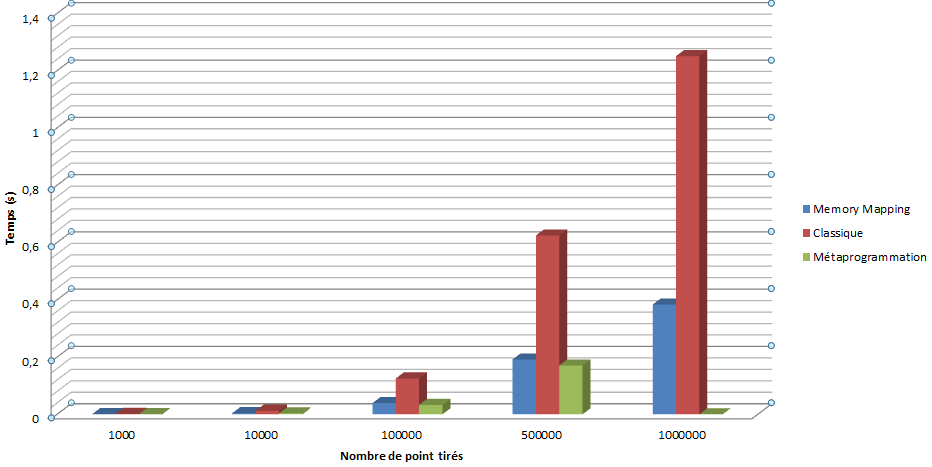
\includegraphics[scale = 0.65]{comparatifResult10.PNG}
   \end{center}
  \caption{Histogramme comparatif des temps d'exécution pour 10 répliques.}
\end{figure}

\normalsize{
{\bf Rappel :} Le métaprogramme ne pouvant pas être compilé pour 1000000 de points et 10 réplications. Nous avons pas pu avoir de résultats pour ce cas là. \\

Ce comparatif montre bien la faiblesse des performances en utilisant la méthode classique. En effet plus le nombre de points tirés est grand plus l'écart relatif avec les autres méthodes est grand (facteur 2,5 pour 100000 points à  facteur 3,5 pour 1000000 de points et à 5 réplications ). Pour ce qui est des performances entre le memory mapping et la métaprogrammation, l'écart est plus réduit ( env 22\% pour 1000000 de points ). Cette différence peut s'expliquer techniquement, l'optimisation à la compilation du tableau de flottant en variable globale permet d'aller plus vite que la projection d'un fichier en mémoire via le memory mapping. 
}

\section{Conclusion}

\normalsize{
Pour conclure sur cette étude de performance et de méthodes alternatives pour obtenir des nombres pseudo-aléatoires, on peut se diviser en deux parties. D'un côté de la performance pure ( du temps d'exécution de la simulation ) la métaprogrammation est la plus efficace des trois testés. D'un autre côté cette méthode demande des ressources énormes pour la mettre en place. Que ce soit à la génération du code source à la compilation, les temps de calcul supplémentaire dépasse largement le gain obtenue à l'exécution. On peut imaginer des cas particuliers où le temps d'exécution est le plus important et qu'on soit pas regardant sur les temps de compilation  où chaque seconde de calcul gagné permet une économie d'énergie importante ( exemple de grille ou de super calculateur). Mais le gros problème de cette méthode est le fait que la liste des nombres aléatoires reste figés. C'est pour cela que le système de memory mapping semble être le meilleur compromis en terme de modularité et de performance. En effet, même si le temps d'exécution est sensiblement supérieur à la métaprogrammation, l'utilisateur peut modifier la liste des nombres aléatoires en entrée.  
}

\chapter{Métamodèle du C++}

\normalsize{
La première partie a porté sur l'utilisation de la métaprogrammation. Cette partie traitera de la métamodélisation. Le but étant de modéliser le langage C++ pour ensuite permettre de générer des headers en C++ puis en java.
}

\section{Modèle d'un attribut}

\normalsize{
Un attribut a besoin pour être modéliser de son type (int, double etc...), de son nom, de son accessibilité (public, privé ou proctected) on peut aussi ajouter des informations comme si c'est un attribut de classe (static) ou d'instance. Ces informations seront stockés dans l'attribut {\bf \_characteristics} ( le détail de l'implémentation sera donnée dans la partie 2.6. Voici la classe Attribut représenté en UML via le logiciel ArgoUML. \\
}

\begin{figure}[!h]
   \begin{center}
   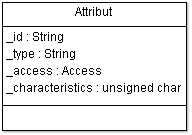
\includegraphics[scale = 1.0]{ModeleAttribut.PNG}
   \end{center}
  \caption{Modèle d'un attribut.}
\end{figure}


\section{Modèle d'une méthode}

\normalsize{
Les méthodes sont un peu plus complexes à modéliser que les attributs. Certes, on peut assimiler le type de retour au type d'un attribut mais une méthode peut être virtuelle ou virtuelle pure en plus d'être statique. Les paramètres de la méthodes peuvent modéliser sous forme de liste de string, leur nom n'est pas nécessaire. Les propriétés (vitual, static etc...) seront stockés dans l'attribut {\bf \_characteristics} comme pour l'attribut.  Voici la classe Methode représenté en UML via le logiciel ArgoUML. \\
}

\clearpage

\begin{figure}[!h]
   \begin{center}
   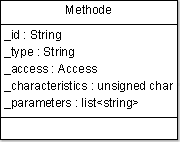
\includegraphics[scale = 1.0]{ModeleMethode.PNG}
   \end{center}
  \caption{Modèle d'une méthode.}
\end{figure}

\section{Factorisation avec des membres}

\normalsize{
On peut remarquer des similitudes entres le modèle de l'attribut et le modèle de la méthode. Il serait judicieux de factoriser ces deux classes par une classe Membre qui contiendrait les attributs communs. Voici sa représentation en langage UML.
}

\begin{figure}[!h]
   \begin{center}
   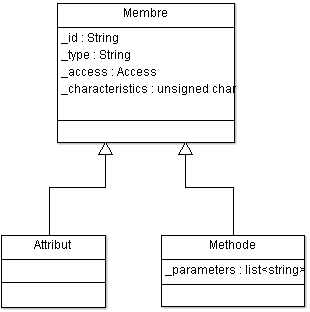
\includegraphics[scale = 0.9]{factorisationUML.PNG}
   \end{center}
  \caption{Factorisation par une classe Membre.}
\end{figure}


\section{Modèle d'une classe}

\normalsize{
Une classe doit être décrite par son nom, les membres qui le constitue, son héritage. Toutes les autres informations ( classe instanciables etc...) peuvent être fourni à l'aide de méthode qui analyseront les membres. Si la classe modélisé spécialise une ou plusieurs classe, il faut connaitre les classes parentes et leur modificateur d'accès. Pour cela on a utilisé une classe d'association contenant un pointeur sur la classe mère ainsi qu'un modificateur d'accès. Voici l'illustration en UML de ce modèle.
}

\clearpage

\begin{figure}[!h]
   \begin{center}
   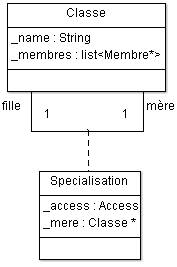
\includegraphics[scale = 0.9]{ModeleClasse.PNG}
   \end{center}
  \caption{Modèle d'une classe .}
\end{figure}


\section{Modèle de l'ensemble}

\normalsize
{
Voici le diagramme assemblé avec les différentes briques décrites ci-dessus.
}

\begin{figure}[!h]
   \begin{center}
   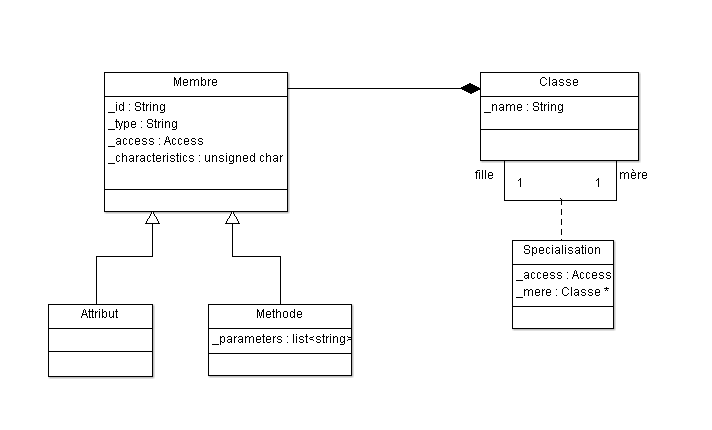
\includegraphics[scale = 0.65]{metamodeleCpp.PNG}
   \end{center}
  \caption{Métamodèle du C++ .}
\end{figure}


\section{Implémentation en C++}

\normalsize{
L'implémentation du métamodèle a été discuté sur deux points, comment modéliser l'accès (private etc...) et comment déterminer les caractéristiques d'un objet. Ces deux points vont être expliquer dans les sous-sections ci-dessous.

\subsection{L'accessibilité}

\normalsize{
Un membre peu être soit privé, soit public , ou public seulement c'est pour cela que la solution d'une {\bf enum} a paru la plus évidente. donc le code modélisant l'accès est le suivant.
}

\begin{lstlisting}[language=C++]
enum Accesibility {
    M_PRIVATE,
    M_PROTECTED,
    M_PUBLIC;
}
\end{lstlisting}

\normalsize{
Avec ce type de code, l'utilisation devient transparente pour l'utilisateur. On pourra taper la ligne suivante pour modifier le type de protection d'un membre.
}

\begin{lstlisting}[language=C++]
monMembre.setAccess(M_PRIVATE); //Pour transformer mon membre en prive.
\end{lstlisting}


\subsection{Les caractéristiques}

\normalsize{
Le problème rencontré avec les caractéristiques est différent que le précédent car une méthode peut à la fois être statique et virtuelle. Donc la solution retenue a été de stocker l'information sur un octet et de travailler sur les bits. Pour cela on utilise des macro pré-processeur comme les suivantes.
}

\begin{lstlisting}[language=C++]
//definition des flags pour les caracteristique du membre
#define M_VIRTUAL      1    //0b001
#define M_PURE_VIRTUAL 3    //0b011 //si virtuelle pure alors deja virtuelle
#define M_STATIC       4    //0b100
\end{lstlisting}

\normalsize{
On l'utilisera comme ceci.
}

\begin{lstlisting}[language=C++]
maMethode.setCharateristics(M_VIRTUAL | M_STATIC); 
//Pour rendre cette methode statique et virtuelle
\end{lstlisting}

\section{Conclusion et améliorations à apporter}

\normalsize{
Ce métamodèle ne prend pas en compte de toute les possibilités du C++ comme les templates, les nested class, les méthodes inline, les struct, les enums etc... et reste simple dans son utilisation. Un approfondissement de la structure qui aurait pu être apporté est la modélisation des types et reprendre une architecture qui se fait en Java ou en Objective-C, c'est à dire du tout objet. Chaque classe serait décrite par une classe. Ce genre de méta modèle serait intéressant dans le sens où on pourrait contrôler toute l'architecture d'un programme et  apporter quelques notions d'introspections au C++. 

Concernant la génération de header en C++, cela n'a pas posé de problèmes car le métamodèle est fait pour le C++. Pour le même fonction en Java, la difficulté a été la différence au niveau de l'héritage. En effet le Java utilise  des interfaces et ne permet pas le multi-héritage. Donc pour notre simple métamodèle, on s'est limité à tester le nombre de parents. Si leur nombre dépassait 1 on envoie une erreur. La solution plus efficace serait de voir parmi les classes parentes, si certaines pourrait devenir des interfaces. Une classe C++ virtuelle pure, sans attributs et sans implémentation des autres classes pourrait être assimiler à une interface. Cependant, une interface Java doit exprimer une capacité (Threadable, Serializable etc...), ce qui pourrait poser problème avec cette solution. 

\chapter{Conclusion}

\normalsize{
Ces deux travaux sont le prolongement de l'étude du premier TP. La première partie est la démonstration de la puissance de la métaprogrammation. La deuxième est l'implémentation d'un métamodèle et de voir une des potentielles applications ( ici la génération de fichiers sources ). \\
}

\normalsize{
Ce qui ressort de la première partie, c'est la possibilité de réduire fortement le temps d'exécution d'une simulation sans passer du temps sur de l'algorithmie ou de l'optimisation de code. La deuxième partie ( métamodélisation ) souligne la difficulté d'avoir une implémentation qui permettrait de faire de l'introspection et de la réflexivité en C++. Ceci étant du à la grande variété du C++ ainsi qu'à la complexité de son architecture qui inclut de nombreux éléments de C qui ne permet pas de faire de l'objet naturellement. On voit bien à travers les solutions de métamodèle plus complet proposé en conclusion que des langages comme le java, l'objective-C ou le C\# sont plus apte à fournir ces mécanismes là. 
}
\end{document}